%pictures and spectra
%tables and graphs
%statements of the result

\section{Results}
\label{sec:Results}

Figure \ref{fig:comparison} shows the normalized resistance of the germanium, copper and nickel samples in a temperature range from $\SI{114.286}{\kelvin}$ up to $\SI{451.038}{\kelvin}$.
The normalizing value is the sample specific resitance at $\SI{0}{\celsius}$.

\begin{figure*}
    \centering
    \captionsetup{width=0.9\linewidth}
    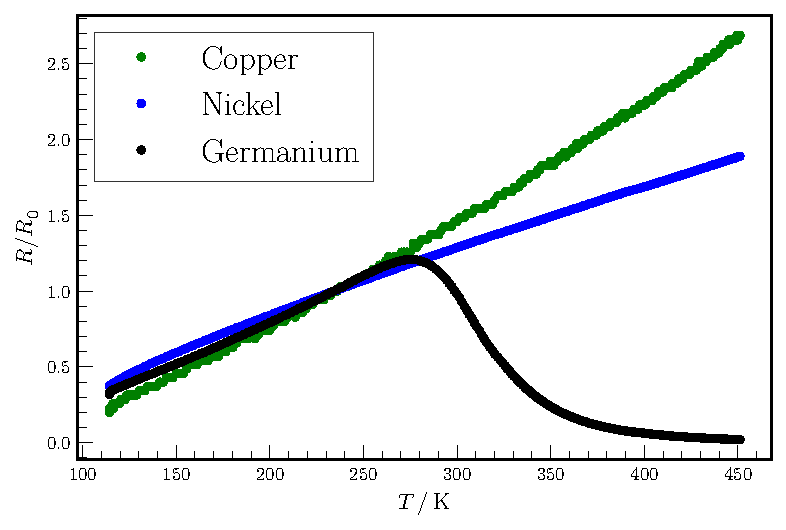
\includegraphics[width=0.7\textwidth]{plots/compare.pdf}
  \caption{Resistance measurement of germanium, copper and nickel, displayed in a nomalized plot based on the resistance at $\SI{0}{\celsius}$.}
    \label{fig:comparison}
\end{figure*}

In figure \ref{fig:metallic-fit} a linear regression in the from
\begin{equation}
    R(T) = R_0 +\beta T
\end{equation}\label{equ:metalic-fit}
has been done and added in the plots. 
As this linear relation describes the metallic behavior, therefore, for the semiconductor only the low temperature data up to a temperature of $\SI{260}{\kelvin}$ have been taken into account.

%% three subfigures next to each others
\begin{figure*}
    \centering
\begin{subfigure}{.45\textwidth}
    \centering
    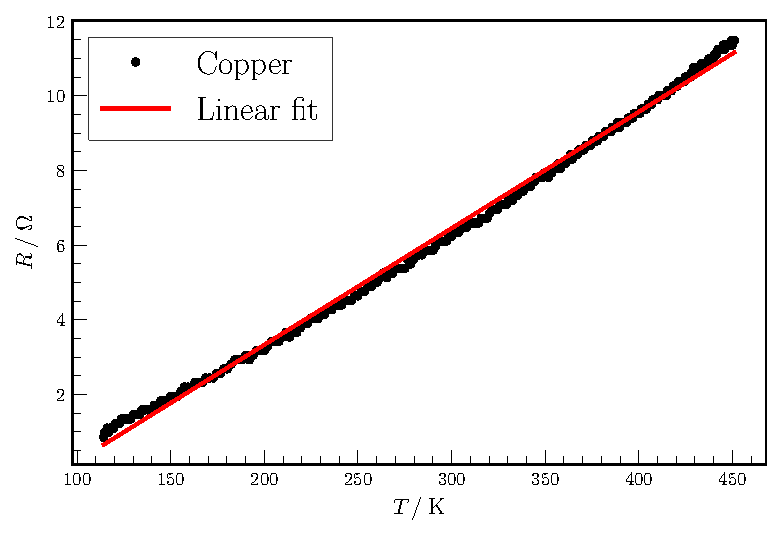
\includegraphics[width=\textwidth]{plots/R2.pdf}
    \caption{Copper}
    \label{fig:Cu}
\end{subfigure}
\begin{subfigure}{.45\textwidth}
    \centering
    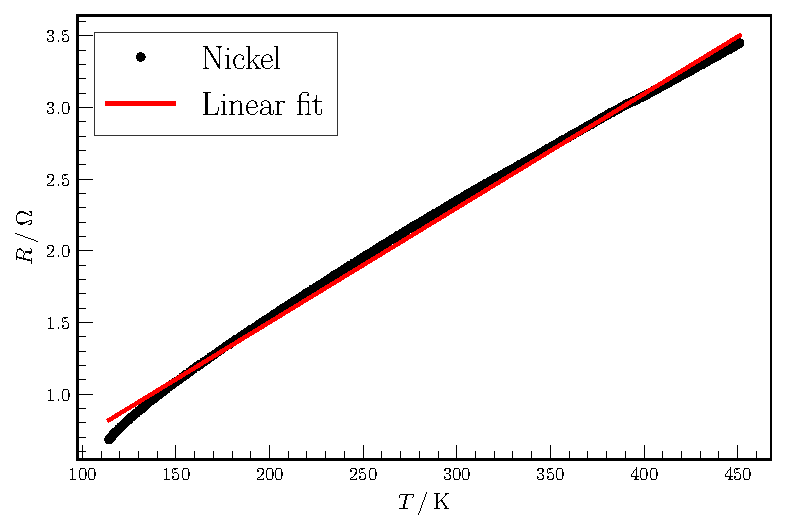
\includegraphics[width=\textwidth]{plots/R3.pdf}
  \caption{Nickel}
    \label{fig:Ni}
\end{subfigure}
\caption{Temperature-dependent resistance of two metallic samples, including a linear regression.}
\label{fig:metallic-fit}
\end{figure*}
%(In the case of germanium only the datapoints with a temperature lower then $\SI{260}{\kelvin}$ have been evaluated.)

The resulting fitting parameters $\beta$ are
\begin{align*}
    \beta(Ge) &= \SI{8.15 \pm 0.04 e-1}{\ohm\per\kelvin} \ref{fig:Ge-exp}\\
    \beta(Cu) &= \SI{3.118 \pm 0.001 e-2}{\ohm\per\kelvin} \\
    \beta(Ni) &= \SI{7.966 \pm 0.001 e-3}{\ohm\per\kelvin} \\
\end{align*}\label{equ:results-beta}

For the semiconductor data, up from a temperature of $\SI{304}{\kelvin}$ an exponential fitting 
\begin{equation}
    R(T) = R_0 e^{-B/T} + C
\end{equation}
has been done, which results in the parameters
\begin{align*}
    R_0 &= \SI{9.05 \pm 0.09 e-3}{\ohm} \\
    B &= \SI{-2936 \pm 29 }{\kelvin} \\
    C &= \SI{-4.27 \pm 0.35 }{\ohm} \\
\end{align*} 

Here, $B$ corresponds to $E_{g,T=0}/2k_b$ (compare equation \ref{eq:intrinsic}) so that the bandgap energy is
\begin{equation}
E_g(Ge,T=0) = B \times 2 k_b = \SI{0.506 \pm 0.005 }{\eV}.
\end{equation}\label{eq:bandgap-exp}

\begin{figure*}
    \centering
\begin{subfigure}{.45\textwidth}
    \centering
    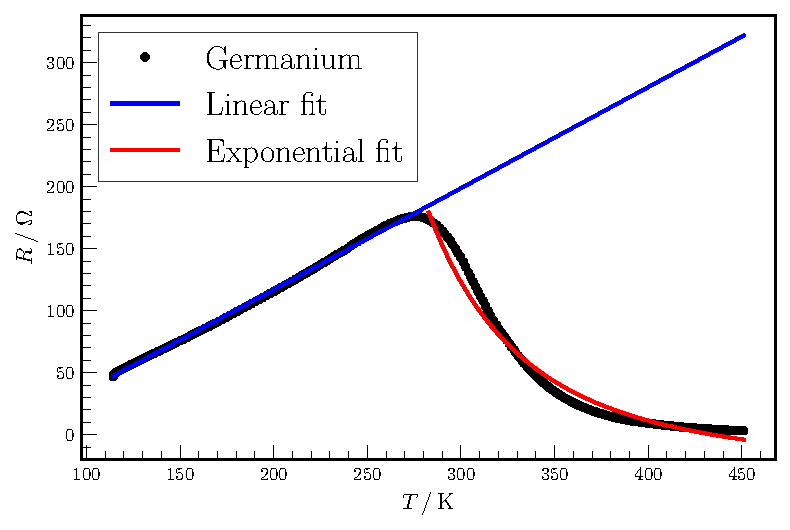
\includegraphics[width=\textwidth]{plots/R1.pdf}
    \caption{Exponential behavior of the resistance for high temperatures higher then $\SI{304}{\kelvin}$.}
    \label{fig:Ge-exp}
\end{subfigure}
\begin{subfigure}{.45\textwidth}
    \centering
    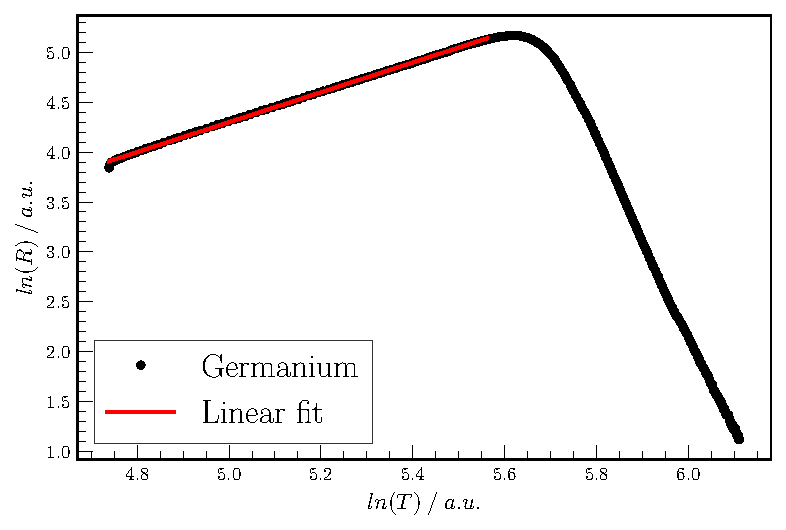
\includegraphics[width=\textwidth]{plots/R1-log.pdf}
  \caption{Double-logarithmic plot with a linear regression for the low temperature regime lower then $\SI{260}{\kelvin}$.}
    \label{fig:Ge-log}
\end{subfigure}
\caption{Temperature-dependent resistance of a germanium sample, with fittings in low and high temperature domain.}
\label{fig:semiconductor-fit}
\end{figure*}

The linear regression in the double-logarithmic plot of resistance against temperature of germanium results in a slope of
\begin{equation}
    \alpha = \num{1.498 \pm 0.004}.
\end{equation}\label{equ:alpha}

\subsection{Resistivity of wires}
\label{sec:res-wires}

The measured diameters $d$ of the four samples are
\begin{align*}
d_A &= \SI{1}{\milli\meter} \\
d_B &= \SI{0.6}{\milli\meter} \\
d_C &= \SI{0.6}{\milli\meter} \\
d_D &= \SI{0.23}{\milli\meter}, \\
\end{align*}
so the used radius $r$ equals $d/2$.

By rearanging the formula \ref{equ:wires} for $R$, a fitting for the pararmter $\rho$ can be obtained.
The resulting resistivities for the 2-wire and 4-wire measurements are given in table \ref{tab:wires}.

\begin{table*}
    \caption{Resistance of four unknown samples obtained by a 2-wire or 4-wire resitance measurement due to a fitting of formula \ref{equ:wires}. The procentual discrepancy, always in the reference of the 4-wire value is added.}
    \label{tab:wires}
    \centering
    \begin{tabular}{l S[table-format=1.3]@{${}\pm{}$}S[table-format=1.2] S[table-format=1.3]@{${}\pm{}$}S[table-format=1.2] S[table-format=3.0]@{${}\pm{}$}S[table-format=3.0]}
          \toprule
          {Sample} & \multicolumn{2}{c}{$\rho_\text{2-wire} \: [\SI{e-6}{\ohm\meter}]$ } & \multicolumn{2}{c}{$\rho_\text{4-wire} \: [\SI{e-6}{\ohm\meter}]$} & \multicolumn{2}{c}{$\text{Deviation} \: [\si{\percent}]$} \\
          \midrule
          {A} & 1.56  & 0.44   & 0.46  & 0.2 & 240 & 170 \\
          {B} & 1.18 & 0.35  & 1.19 & 0.05 & 1 & 30\\
          {C} & 0.353  & 0.09 & 0.20  & 0.05 & 80 & 60 \\
          {D} & 0.110  & 0.026   & 0.046  & 0.002 & 140 & 60 \\
          \bottomrule
    \end{tabular}
\end{table*}

% Seeing the big procentual discrepancy between the estinated value between the 2-wire- and 4-wire-measurement it becomes clear how big the quality of the measurement can be, especially as a low resisitvity material as a metal is to been analyzed.
% Therfore, in order to estimate the material, only the 4-wire-measurement data are taken into account.
% Comparing the obtained resistivities with literature, oner comes to the estimate that sample B may be magnese ($\rho=\SI{144e-8}{\ohm\meter}$)\cite{lead}, sample C may be lead ($\rho=\SI{22e-8}{\ohm\meter}$)\cite{lead} and sample D may be copper ($\rho=\SI{1.68e-8}{\ohm\meter}$)\cite{copper}.
% Here, the procentual deviation is 
% \begin{align*}
%     \delta \rho_\text{B-Mg} &= \SI{100}{\percent} \\
%     \delta \rho_\text{C-Pb} &= \SI{100}{\percent} \\
%     \delta \rho_\text{D-Co} &= \SI{100}{\percent} .\\
% \end{align*}

